%%----------------------------------------------------------------------------
%% Presentatie HoGent Bedrijf en Organisatie
%%----------------------------------------------------------------------------
%% Auteur: Bert Van Vreckem [bert.vanvreckem@hogent.be]

\documentclass{beamer}

%==============================================================================
% Aanloop
%==============================================================================

%---------- Packages ----------------------------------------------------------
\usepackage{etex}
\usepackage{graphicx,multicol}
\usepackage{comment,enumerate,hyperref}
\usepackage{amsmath,amsfonts,amssymb}
\usepackage{tikz}
\usepackage[dutch]{babel}
\usepackage[utf8]{inputenc}
\usepackage{multirow}
\usepackage{eurosym}
\usepackage{listings}
\usepackage[T1]{fontenc}
\usepackage{lmodern}
\usepackage{textcomp}
\usepackage{framed}
\usepackage{wrapfig}
\usepackage{pgf-pie}
\usepackage{pgfplots}
\usepackage{booktabs}
\usepackage{pgfplotstable}
\usepackage{changepage}
\usepackage{pst-plot,pst-func}

%---------- Configuratie ------------------------------------------------------

\usetikzlibrary{arrows,shapes,backgrounds,positioning,shadows}
\usetikzlibrary{pgfplots.statistics}


\usetheme{hogent}
\setbeameroption{show notes}

%---------- Commando-definities -----------------------------------------------

\newcommand{\tabitem}{~~\llap{\textbullet}~~}
\renewcommand{\arraystretch}{1.2}

%---------- Info over de presentatie ------------------------------------------

\title[Intro]{Research Techniques\\$\chi^{2}$ test}
\author{Wim Goedertier, Jens Buyse, Bert {Van Vreckem}, Wim {De Bruyn}}
\date{AY 2017-2018}

%==============================================================================
% Inhoud presentatie
%==============================================================================

\begin{document}

%---------- Front matter ------------------------------------------------------

% Dia met het HoGent logo
\HoGentLogo

% Titeldia met faculteitslogo
\titleframe

%---------- Inhoud ------------------------------------------------------------

\pgfmathdeclarefunction{gauss}{2}{%
  \pgfmathparse{1/(#2*sqrt(2*pi))*exp(-((x-#1)^2)/(2*#2^2))}%
}



\begin{frame}
  \frametitle{What's on the menu today?}

  \tableofcontents
\end{frame}

\begin{frame}
  \frametitle{Recap}

  \begin{itemize}
    \item What is a hypothesis?
    \item What components does a hypothesis test consist of?
    \item What is the procedure of a hypothesis test?
    \item Which errors can be made?
  \end{itemize}
\end{frame}

\section{$\chi^{2}$ test for one variable}
\sectionframelogo{}

\begin{frame}
  \frametitle{Goodness of fit test}
  \brightbox{A \textcolor{HoGentAccent6}{goodness of fit test} can be used to determine to what extent a sample conforms to a null hypothesis about the distribution of a variable.}

  \begin{columns}
    \begin{column} {0.5\textwidth}

    \begin{figure}
      \centering
        
\includegraphics[width=0.8\textwidth]{img/les6-man.jpg}
    \end{figure}

    \end{column}
    \begin{column} {0.5\textwidth}

    \begin{figure}
      \centering
        
\includegraphics[width=1.00\textwidth]{img/les5-heroes.jpg}
    \end{figure}

    \end{column}
  \end{columns}
\end{frame}

\begin{frame}
  \frametitle{Goodness of fit test}
  We want to check whether the distribution of superhero types in our sample of $n = 400$ conforms to the expected distribution in the population (all superheroes) as a whole.
  
  \begin{itemize}
    \item Compare numbers in the sample with expected values if the sample is completely representative
    \item ``Large'' differences $\Rightarrow$ the distribution of the sample doesn't match
    \item ``Small'' differences $\Rightarrow$ the distribution matches
  \end{itemize}

  \pause
  Can you see a resemblance to contingency tables and Cramer's V?
\end{frame}

\begin{frame}
  \frametitle{Goodness of fit test}
  \begin{columns}
    \begin{column} {0.2 \textwidth}

    \begin{figure}
      \centering
        
\includegraphics[width=\textwidth]{img/les6-man.jpg}
    \end{figure}

    \end{column}

    \begin{column} { 0.8 \textwidth}
    \begin{table}
\begin{tabular}{lcc}
	\toprule
	\textbf{Type} & \textbf{\# in sample} & \textbf{\% in population} \\
	              & \emph{o}              & $\pi$                     \\ \midrule
	Mutant        & 127                   & 35\%                      \\
	Human         & 75                    & 17\%                      \\
	Alien         & 98                    & 23\%                      \\
	God           & 27                    & 8\%                       \\
	Demon         & 73                    & 17\%                      \\ \bottomrule
\end{tabular}
\end{table}
    \end{column}
  \end{columns}
\end{frame}

\begin{frame}
  \frametitle{Goodness of fit test}
  
  \begin{itemize}
    \item We want to know if the sample is representative
    \item If sample is exactly representative $\Rightarrow$ 35\% of superheroes in the sample should be a mutant
    \item The expected number is $0.35 \times 400 = 140$.
    \item Notation: $e$ (expected).
  \end{itemize}

  \[ e = n \times \pi \]
  
  If the differences $o - e$ are relatively small, they can be attributed to random sample errors.
\end{frame}

\begin{frame}
  \frametitle{Goodness of fit test}
  Beschouw $\chi^{2}$:

  \[ \chi^{2} = \sum_{i=1}^{n} \frac{(o_{i} - e_{i})^{2}}{e_{i}} \]

  Remarks:
  \begin{itemize}
    \item if the differences are sufficiently small $\Rightarrow$ distribution matches
    \item if the differences are too large $\Rightarrow$ distribution doesn't match
  \end{itemize}
  
  $\chi^{2}$ measures the difference of the observed values with the null hypothesis
\end{frame}

\begin{frame}
  \frametitle{Goodness of fit test}
  \begin{columns}
    \begin{column} {0.2 \textwidth}

    \begin{figure}
      \centering
        
\includegraphics[width=\textwidth]{img/les6-man.jpg}
    \end{figure}

    \end{column}

    \begin{column} { 0.8 \textwidth}
      % Please add the following required packages to your document preamble:
% \usepackage{booktabs}
\begin{table}[h]
\begin{tabular}{@{}llllll@{}}
\toprule
\textbf{Superhero type} & \textbf{$o$} & \textbf{$\pi$} & \textbf{$e$} & \textbf{$o -e$} & \textbf{$\frac{(o-e)^{2}}{e}$} \\ \midrule
Mutant                  & 127          & 35\%           & 140          & -13             & 1.21                           \\
Human                    & 75           & 17\%           & 68           & 7               & 0.72                           \\
Alien                   & 98           & 23\%           & 92           & 6               & 0.39                           \\
God                     & 27           & 8\%            & 32           & -5              & 0.78                           \\
Demon                   & 73           & 17\%           & 68           & 5               & 0.37                           \\ \bottomrule
 & 400 & & 400 & & 3.47 \\
\end{tabular}
\end{table}
    \end{column}
  \end{columns}
  \[ \chi^{2} = \sum_{i=1}^{n} \frac{(o_{i} - e_{i})^{2}}{e_{i}} = 3.47\]
\end{frame}


\begin{frame}
  \frametitle{Goodness of fit test}
    The test statistic $\chi^{2}$ follows the $\chi^{2}$ distribution\\
    The shape of the $\chi^{2}$ distribution depends on the $df$ parameter
\vfill
    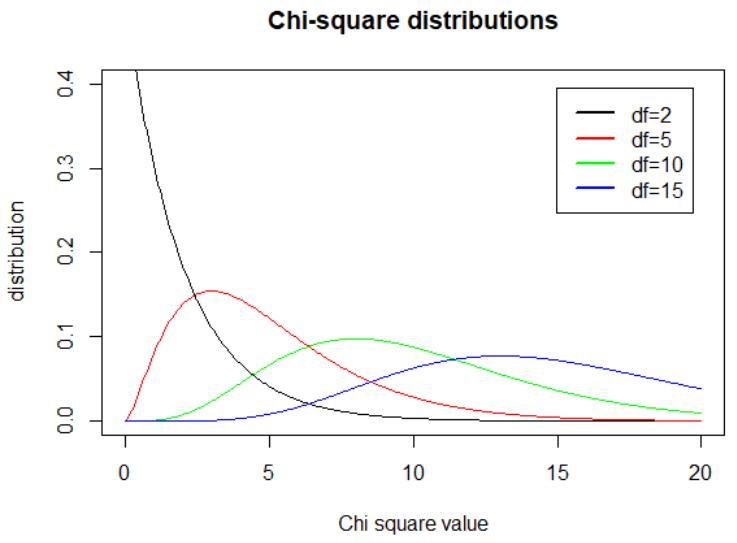
\includegraphics[width=0.8\textwidth]{img/chap6-chi-square-distributions.png}
\end{frame}

\begin{frame}
\frametitle{Goodness of fit test}

\begin{itemize}
    \item The critical value $b$ for a specified significance level $\alpha$ and a specific degrees of freedom $df$ can be looked up in a table, or calculated in R.
\vfill
    \item The degrees of freedom ($df$) are defined by:
    \[ df = k -1 \]
    with $k$ the number of categories
\vfill 
    \item $b = \texttt{qchisq}(1-\alpha,k-1)$
    \item $\alpha = 1-\texttt{pchisq}(b,k-1)$
\end{itemize}
\end{frame}

\subsection{Test procedure goodness of fit test}

\begin{frame}
  \frametitle{Test procedure goodness of fit test}
  \begin{enumerate}
  \item \textbf{Formulate hypotheses}
    \begin{itemize}
      \item $H_{0}$: sample is representative for the population
      \item $H_{1}$: sample is \emph{not} representative for the population
    \end{itemize}
  \item \textbf{Determine $\alpha$, $n$ and $df$}
  \item \textbf{Calculate test statistic}
  \[ \chi^{2} = \sum_{i=1}^{n} \frac{(o_{i} - e_{i})^{2}}{e_{i}} \]
  \item \textbf{Calculate critical value $b$ or $p$-value}\\
  Remark: $\chi^2$ tests are \emph{always} right-tailed.
  \item \textbf{Conclusion}\\
   If $\chi^2 < g$ (or $p > \alpha$) : accept $H_{0}$\\
   If $\chi^2 > g$ (or $p < \alpha$) : reject $H_{0}$ and accept $H_{1}$.
\end{enumerate}
\end{frame}

\begin{frame}
\frametitle{Test procedure goodness of fit test (example)}
\begin{enumerate}
    \item \textbf{Formulate hypotheses}
      \begin{itemize}
        \item $H_{0}$: sample is representative for the superhero population
        \item $H_{1}$: sample is \textbf{\emph{not}} representative for the population
      \end{itemize}
    \item \textbf{Determine $\alpha$, $n$ and $df$}
        \[ \alpha = 0.05 , n = 400, df = 5-1 = 4 \]
    \item \textbf{Calculate test statistic}:
        \[ \chi^{2} = 3.47 \]
    \item \textbf{Calculate critical value $b$ or $p$-value}
      \begin{itemize}
        \item $b = \texttt{qnorm}(0.95,4) = 9.49$
        \item $p = 1-\texttt{pnorm}(3.47) = 0.48 = 48\%$
      \end{itemize}
    \item \textbf{Conclusion}\\
    ~~~~$3.47 < 9.49$ (or $48\% > 5\%$) : $H_0$ is accepted\\
    ~~~~we have a very representative sample
\end{enumerate}
\end{frame}

\subsection{Example}

\begin{frame}
  \frametitle{Example: family composition}
  
  Consider all families with 5 children in a certain community,\\
  where the expected probability of getting a boy is equal to that of a girl (i.e. 50\%)
  \vfill
  \pause
  There are 6 possible family compositions:
  \begin{enumerate}
    \item 0 boys, 5 girls
    \item 1 boy, 4 girls
    \item 2 boys, 3 girls
    \item 3 boys, 2 girls
    \item 4 boys, 1 girl
    \item 5 boys, 0 girls
  \end{enumerate}

\end{frame}

\begin{frame}
  \frametitle{Example: family composition}
  Are the observed values ($o_i$) in a survey of 1022 families with 5 kids representative for this community?
  \begin{table}[h]
\begin{tabular}{@{}rrrrrrrr@{}}
\toprule
$i$ (\#boys)         & 0  & 1   & 2   & 3   & 4   & 5  &  \\ \midrule
$o_{i}$ (\#families) & 58 & 149 & 305 & 303 & 162 & 45 &  \\ \bottomrule
\end{tabular}
\end{table}
\pause
The probability $\pi_{i}$ to have $i$ boys in a family of 5 is determined by a binomial distribution with parameters $n=5$ and $p=0.5$. E.g. the probability for 2 boys is:

\[ (0.5)^{2} \times (1-0.5)^{5-2} \times \binom{5}{2} \]

In general:

\[ \pi_{i} = \binom{5}{i}\times p^{i} \times p^{5-i} = \frac{5!}{i!(5-i)!}\times 0.5^{i} \]
\end{frame}

\begin{frame}
  \frametitle{Example: family composition}
  \begin{table}[h]
\begin{tabular}{@{}llllllll@{}}
\toprule
$i$                         & 0        & 1        & 2        & 3        & 4       & 5       & $\Sigma$\\ \midrule
$o_i$                      & 58       & 149      & 305      & 303      & 162     & 45      & 1022    \\
$\pi_i$                      & 0.03    & 0.15    & 0.31    & 0.31  & 0.15 & 0.031 & 1       \\
$e_i$                      & 31.68   & 159.43  & 318.86  & 318.86  & 159.43 & 31.68  &         \\
$\frac{(o-e)^{2}}{e}$ & 21.86 & 0.68259  & 0.60   & 0.78  & 0.041 & 5.59 & 29.57 \\
$r_i$                      & 4.74   & -0.89 & -0.93 & -1.07106 & 0.22 & 2.40 &         \\ \bottomrule
\end{tabular}
\end{table}
\end{frame}

\begin{frame}
  \frametitle{Example: family composition}
  \begin{enumerate}
  \item \textbf{Formulate hypotheses}
    \begin{itemize}
      \item $H_{0}$: sample is representative for the population
      \item $H_{1}$: sample is \emph{not} representative for the population
    \end{itemize}
  \item \textbf{Determine $\alpha$ and $n$} : $\alpha = 0.01$ and $n = 1022$.
  \item \textbf{Calculate test statistic for sample}:
  \[ \chi^{2} = \sum_{i=1}^{n} \frac{(o_{i} - e_{i})^{2}}{e_{i}} = 29.5766 \]
  \item \textbf{Calculate critical value}: $g = 15.0863$. Our test statistic lies within the critical area, and we can reject $H_{0}$. The sample is \emph{not} representative.
\end{enumerate}
\end{frame}

\subsection{Standardised residuals}
\begin{frame}
  \frametitle{Standardised residuals}
  \brightbox{The \textcolor{HoGentAccent6}{Standardised residuals} indicate which categories contribute the most to the value of the statistic.}
  \[ r_{i} = \frac{o_{i} - e_{i}}{\sqrt{e_{i}(1-\pi_{i})}} = \frac{o_{i} - n \pi_{i}}{\sqrt{n \pi_{i}(1-\pi_{i})}} \]

  \begin{itemize}
    \item Rule of thumb: values with $|r_i| > 2$ are considered to be extreme
  \end{itemize}

  We can conclude that the number of families with only boys or only girls is larger than expected.
\end{frame}

\begin{frame}
  \frametitle{Conditions}
  \textbf{Rule of Cochran:}\\
  In order to be allowed to apply the $\chi^2$-test, the following conditions must be observed: 
  \begin{enumerate}
    \item expected value $e$ must be $>1$ for all categories
    \item expected value $e$ must be $\ge5$ for 80\% of all categories
  \end{enumerate}
\end{frame}

\section{$\chi^{2}$ test for two variables}
\sectionframelogo{}

\begin{frame}
  \frametitle{$\chi^{2}$ test for two variables}
  The Chi-squared test can also be applied on a research question regarding two variables.
\vfill
  The approach is exactly the same, but the degree of freedom will now be defined as:
 \[ df = (r-1) \cdot (k-1) \]
  with $r$ the number of levels/categories of one variable\\
  and $k$ the number of levels/categories of the other variable.
\end{frame}

\begin{frame}
  \frametitle{Example: smoking doctors}
  
  Doll and Hill researched the relation between smoking and lung cancer. In 1951, they sent a letter to all British general practicioners with the request to provide data about their age and smoking behaviour.
  
  Next, they observed obituaries and causes of death for years on end. The first results, after about 4 years, are summarised below:

  \begin{table}[h]
    \begin{tabular}{@{}lllll@{}}
    	\toprule
    	                & \textbf{Lung cancer} & \textbf{No} & \textbf{Yes} & \textbf{Total} \\ \midrule
    	\textbf{Smoker} & \textbf{Yes}         & 21178       & 83           & 21261          \\
    	                & \textbf{No}          & 3092        & 1            & 3093           \\
    	                & \textbf{Total}       & 24270       & 84           & 24354          \\ \bottomrule
    \end{tabular}
  \end{table}
\end{frame}

\begin{frame}
  \frametitle{Example: smoking doctors}
  \begin{table}[h]
    \begin{tabular}{@{}lllll@{}}
      \toprule
            & \textbf{Lung cancer} & \textbf{No} & \textbf{Yes} & \textbf{Total} \\ \midrule
      Smoker & Yes                  & 21178       & 83           & 21261          \\
            & No                   & 3092        & 1            & 3093           \\
            & Total                & 24270       & 84           & 24354          \\ \bottomrule
    \end{tabular}
  \end{table}

  \begin{columns}
    \begin{column}{0.3 \textwidth}
  
    \begin{figure}
      \centering
        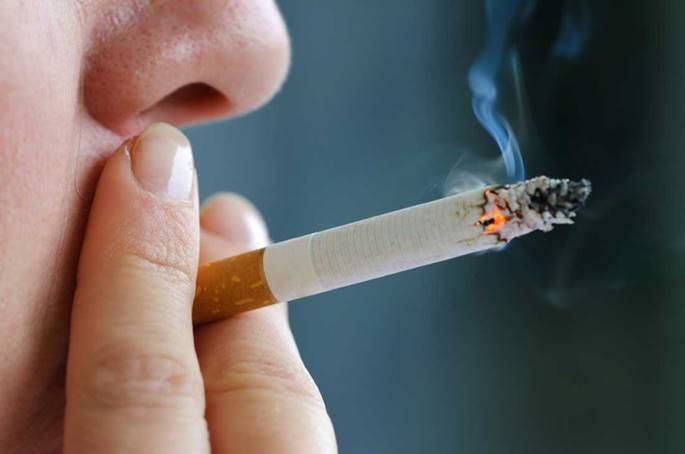
\includegraphics[width=1.00\textwidth]{img/les-6-smoking.jpg}
    \end{figure}
  
    \end{column}
    \begin{column}{0.7 \textwidth}
  
    \begin{itemize}
      \item \dots only $\frac{84}{ 24354} \times 100 = 0.35\% $ of British doctors died of lung cancer
      \item \dots only $\frac{83}{21261} \times 100 = 0.39\%$ of those were smokers
      \item \dots but this is much larger than the number of non-smokers $\frac{1}{3093} * 100 = 0.032\%$.
    \end{itemize}
    \end{column}
  \end{columns}
\end{frame}

\begin{frame}
  \frametitle{Example: smoking doctors, expected values}
  
\begin{table}[h]
\begin{tabular}{@{}lllll@{}}
\toprule
      & \textbf{Lung cancer} & \textbf{No} & \textbf{Yes} & \textbf{Total} \\ \midrule
Smoker & Yes                 & 21188         & 73.3         & 21261           \\
      & No                & 3082.3        & 10.7         & 3093            \\
      & Total              & 24270         & 84           & 24354           \\ \bottomrule
\end{tabular}
\end{table}

\begin{columns}
  \begin{column}{0.3 \textwidth}

  \begin{figure}
    \centering
      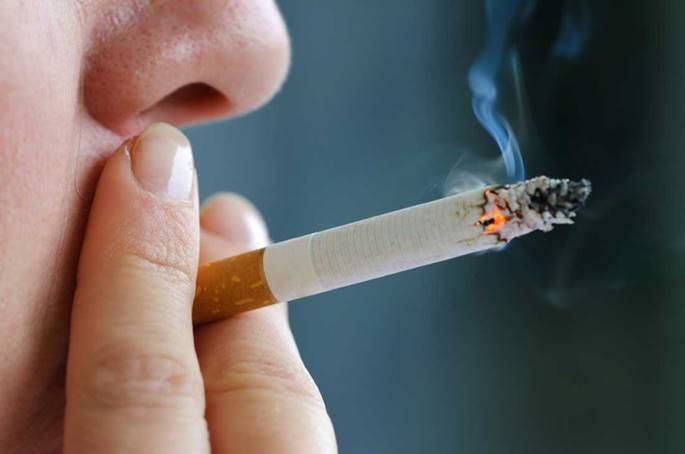
\includegraphics[width=1.00\textwidth]{img/les-6-smoking.jpg}
  \end{figure}

  \end{column}
  \begin{column}{0.7 \textwidth}

  \begin{itemize}
    \item $\chi^{2} = 10.35$
    \item Large difference between observed and expected number of smokers who died from lung cancer
    \item The same goes for the limited number of doctors that were not smokers, but did die from lung cancer
  \end{itemize}
  \end{column}
\end{columns}
\end{frame}

\begin{frame}
  \frametitle{Example: smoking doctors}
  \begin{enumerate}
  \item \textbf{Formulate hypotheses}
    \begin{itemize}
      \item $H_{0}$: there is no relation between the dependent and independent variable
      \item $H_{1}$: there \emph{is} a relation between them
    \end{itemize}
  \item \textbf{Determine $\alpha$ and $n$} : $\alpha = 0.05$ and $n = 24354$.
  \item \textbf{Calculate test statistic in the sample}:
  \[ \chi^{2} = \sum_{i=1}^{n} \frac{(o_{i} - e_{i})^{2}}{e_{i}} = 10.35 \]
  \item \textbf{Calculate critical value}: the critical value is $g = 3.8415$ and the degrees of freedom is $df = (r-1)(k-1) = 1$. The test statistic lies within the critical area, so we reject $H_{0}$.
\end{enumerate}
\end{frame}

\begin{frame}
  \frametitle{Causal relation}
  
  The conclusion is that smokers die from lung cancer more often than non-smokers. However, this does not prove a \emph{causal} relation!
  
  \begin{columns}
    \begin{column}{0.3 \textwidth}
  
      \begin{figure}
        \centering
          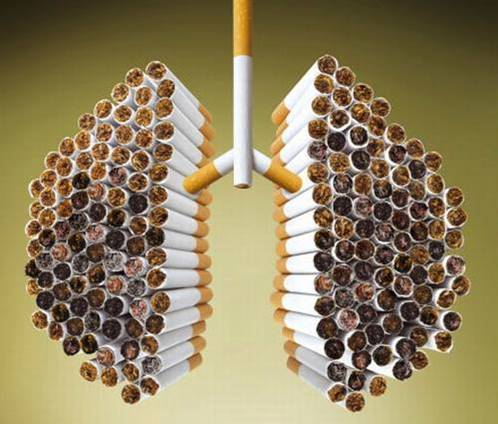
\includegraphics[width=1.00\textwidth]{img/les-6-smoking2.jpg}
      \end{figure}
  
    \end{column}
    \begin{column}{0.7 \textwidth}
  
      \begin{itemize}
        \item \dots not all smokers get lung cancer
        \item \dots the smokers rokers could be older than the non-smokers
        \item \dots more smokers live in the large cities with more air pollution
        \item \dots a genetic disposition could have influence both on tobacco addiction and the probability to get lung cancer
      \end{itemize}
    
    \end{column}
  \end{columns}

  For a causal interpretation of the data (this was \emph{not} an experiment!), we at least need a theory that explicitly models the relation between smoking and lung cancer.
\end{frame}

\end{document}
